%% main.tex — IEEE Conference (IEEEtran), Türkçe
%% Derleme: pdflatex main && bibtex main && pdflatex main && pdflatex main
%% Şekiller: paper/figures/ (python paper/build_paper_figures.py)

\documentclass[conference,a4paper]{IEEEtran}

\usepackage[utf8]{inputenc}
\usepackage[T1]{fontenc}
\usepackage{graphicx}
\usepackage{amsmath}
\usepackage{amssymb}
\usepackage{booktabs}
\usepackage{cite}
\usepackage{placeins}
\usepackage[turkish]{babel}

\addto\captionsTurkish{\renewcommand{\abstractname}{Özet}}
\renewcommand{\IEEEkeywordsname}{Anahtar Kelimeler}

\title{Knapsack (Sırt Çantası Problemi)}

\author{
\IEEEauthorblockN{İrem Kaya -- 232803060}
\IEEEauthorblockA{
Manisa Celal Bayar Üniversitesi\\
Yazılım Mühendisliği Bölümü
}
}

\begin{document}
% Turkish babel may make '=' active; breaks graphicx keyval (width=\columnwidth).
\shorthandoff{=}

\renewcommand{\refname}{Kaynakça}

\maketitle

\begin{abstract}
Bu bildiride 0/1 sırt çantası problemi için önce dinamik programlama (DP) ile kesin çözüm, ardından aynı veri kümelerinde tümlenmiş tavlama (SA) ile yaklaşık çözüm ele alınmıştır. $N \in \{100,\,1000,\,10\,000\}$ boyutlarında çalışma süresi ve (DP tamamlandığında) SA'nın DP optimumuna göre doğruluk açığı raporlanmıştır. Greedy ve Greedy-SA ek sezgisel karşılaştırma olarak çalıştırılmıştır. DP, $N{=}100$ ve $N{=}1000$ için optimum referans üretmiş; $N{=}10\,000$ için 1800 saniyelik sınırda \texttt{timeout} olmuş ve bu boyutta gap hesaplanamamıştır. SA tüm boyutlarda kısa sürede uygulanabilir yaklaşık çözüm döndürmüştür.
\end{abstract}

\begin{IEEEkeywords}
knapsack, dinamik programlama, tümlenmiş tavlama, doğruluk açığı, ölçeklenebilirlik.
\end{IEEEkeywords}

\section{Giriş}

\subsection{Knapsack Probleminin Tanımı}
Sırt çantası (knapsack) problemi, sınırlı kapasite altında seçilecek nesnelerin toplam faydasını (değerini) en büyüklemeyi amaçlayan temel bir ayrık karar modelidir. Uygulamada her nesne genellikle bir ağırlık (kaynak tüketimi) ve bir değer (kazanç veya fayda) ile temsil edilir; çanta veya konteyner ise sabit bir üst kapasite ile modellenir. Karar, hangi nesnelerin bir arada seçileceğidir; klasik \emph{0/1} sürümünde her nesne ya tamamen dahil edilir ya da hiç seçilmez, yani kesirli miktarlar söz konusu değildir. Bu yapı, ``ya tam al ya da alma'' biçimindeki yatırım, proje seçimi veya yük bindirme kararlarının soyut bir örneğidir. Problem, tek bir kapasite kısıtı altında ikili kararların birleşik etkisini incelemeyi sağladığından, hem eğitim hem de araştırma bağlamında optimizasyon ve işlem araştırması derslerinin sık kullanılan bir konusudur \cite{martello1990knapsack}.

\subsection{Problemin Matematiksel Temelleri}
$n$ nesne indekslensin. Her $i$ için $w_i$ ağırlığı, $v_i$ değeri ve toplam kapasite $C$ pozitif ve gerçekçi üst sınır olarak verilir. 0/1 karar değişkeni $x_i \in \{0,1\}$, $i$ nesnesinin seçilip seçilmediğini gösterir. Amaç fonksiyonu toplam değeri $\sum_i v_i x_i$ en büyüklemek; kısıt ise seçilen nesnelerin toplam ağırlığının kapasiteyi aşmaması, yani $\sum_i w_i x_i \leq C$ şeklindedir. Böylece problem, tamsayı doğrusal programlama ve birleşik iyileştirme literatürünün doğal bir üyesi olarak formüle edilir; çözüm uzayı $\{0,1\}^n$ üzerinde tanımlıdır. Aşağıdaki Yöntem bölümünde bu model denklem biçiminde tekrar verilmiş ve deneylerde kullanılan ölçütler bu tanımla uyumludur.

\subsection{Çözüm Zorlukları ve NP-Zor Yapı}
$n$ arttıkça olası 0/1 seçim vektörlerinin sayısı $2^n$ ile üstel büyüdüğünden, tüm kombinasyonları tek tek denemek büyük $n$ için uygulanamaz hale gelir. Knapsack, Karp'ın klasik çalışmasında da yer alan NP-zor problemler arasındadır \cite{karp1972reducibility}; bu, genel durumda polinom zamanda kesin ve her örnek için doğru çalışan bir algoritma beklemenin zor olduğu anlamına gelir. Buna karşın, kapasite $C$ göreli olarak sınırlı kaldığında dinamik programlama gibi yöntemler pseudo-polynomial sürede kesin çözüm üretebilir; maliyet tipik olarak $n$ ve $C$ ile birlikte büyür. Pratikte hem $n$ hem $C$ büyüdüğünde bellek ve süre baskısı artar; tam yöntem aynı teorik kesinliği korusa da duvar saati açısından sonuç döndüremeyebilir. Bu nedenle, kısa sürede uygulanabilir çözüm arayan sezgisel ve meta-sezgisel yaklaşımlar, özellikle büyük örneklerde önem kazanır \cite{kellerer2004knapsack}.

\subsection{Gerçek Hayattaki Kullanım Alanları}
Knapsack soyutlaması, yalnızca akademik bir egzersiz olmayıp birçok karar destek senaryosunun çekirdeğini oluşturur. Örneğin yükleme ve lojistikte sınırlı taşıma kapasitesi altında kârlı yük seçimi, bütçe kısıtı altında proje veya yatırım portföyü seçimi, sınırlı işlemci veya bant genişliğinin paylaştırılması, kesme--paketleme problemlerinin gevşetilmiş formları ve kaynak tahsisi modelleri, kapasite üstü ve ikili seçim yapısıyla knapsack ile ilişkilendirilebilir \cite{martello1990knapsack,kellerer2004knapsack}. Bu çalışmada ele alınan deneysel düzen, bu tür modellerin ortak matematiksel iskeletini yansıtan standart bir test ortamıdır; sonuçlar doğrudan tek bir endüstri kaydına bağlanmadan, ölçeklenebilirlik ve doğruluk açısından yorumlanır.

\subsection{Bu Çalışmanın Amacı}
Bu bildirinin odağı, \emph{aynı} üretilmiş veri üzerinde kesin çözüm üreten dinamik programlama (DP) ile yaklaşık çözüm üreten tümlenmiş tavlama (SA) yöntemlerinin $N \in \{100,\,1000,\,10\,000\}$ boyutlarında çalışma süresi ve (mümkün olduğunda) DP'ye göre doğruluk açığı açısından karşılaştırılmasıdır. Greedy ve Greedy-SA yalnızca ek sezgisel karşılaştırma olarak raporlanmıştır. DP, $N{=}10\,000$ için duvar saati sınırında \texttt{timeout} ile sonuçlanabileceği protokol ile çalıştırılmış; bu durumda optimum bilinmediğinden SA için gap raporlanmaz.

\section{Literatür Taraması}

\textbf{Bellman (1957):} Richard Bellman'ın dinamik programlama eseri, bir optimizasyon problemini daha küçük alt problemlere bölmenin ve optimum değer fonksiyonunun geriye doğru veya ileriye doğru inşasının genel ilkesini ortaya koymuştur \cite{bellman1957dynamic}. Bu çerçeve, knapsack gibi ayrık karar modellerinde tablo tabanlı kesin yöntemlerin kuramsal dayanağını sağlar. Özellikle alt problemler arasındaki yineleme ilişkisi, DP'nin neden kesin optimum verebildiğini açıklar. Knapsack literatüründe klasik DP gerçekleştirmeleri bu gelenek içinde yer alır.

\textbf{Martello ve Toth (1990):} Martello ve Toth'un monografisi, knapsack ailesindeki problem sınıflarını, tam ve sezgisel algoritmaları ve uygulama odaklı tartışmaları bir araya getiren temel bir başvuru kaynağıdır \cite{martello1990knapsack}. Kitap, farklı knapsack varyantlarının karmaşıklığını ve pratikte hangi yöntem sınıflarının tercih edilebileceğini sistematik biçimde ele alır. Bu çalışmadaki problem tanımı ve karşılaştırmalı deneysel bakış açısı, bu kaynakla uyumlu bir çerçevede anlaşılabilir.

\textbf{Kellerer, Pferschy ve Pisinger (2004):} Kellerer, Pferschy ve Pisinger'in knapsack kitabı, konunun modern ve geniş kapsamlı bir sentezini sunar \cite{kellerer2004knapsack}. Teorik alt sınırlar, tam algoritmalar, yaklaşık çözümler ve deneysel değerlendirme pratikleri birlikte işlenir. Büyük kapasite veya büyük $n$ durumunda tam yöntemlerin pratik sınırları ile sezgisel yöntemlerin rolü bu eserde vurgulanır; bizim ölçeklenebilirlik odaklı deney tasarımımız bu tartışmayla ilişkilidir.

\textbf{Kirkpatrick, Gelatt ve Vecchi (1983):} Kirkpatrick, Gelatt ve Vecchi'nin Science makalesi, tümlenmiş tavlamayı fiziksel tavlama benzetmesiyle açıklayarak komşu çözümlere geçişte kötüleşen hamlelerin belirli bir sıcaklık parametresiyle olasılıksal olarak kabul edilebileceğini göstermiştir \cite{kirkpatrick1983optimization}. Bu mekanizma, yerel optimumlardan kaçışı destekleyen genel bir meta-sezgisel çerçeve sunar. Bizim SA uygulamamız, bu ilkeye dayanan yaklaşık bir arama yöntemi olarak konumlanır.

\textbf{Glover ve Kochenberger (2003):} Glover ve Kochenberger'ın editörlüğündeki meta-sezgisel el kitabı, SA dahil birçok yöntemin tasarım ilkelerini ve uygulama alanlarını geniş bir perspektifle toplar \cite{glover2003handbook}.

\section{Yöntem}

\subsection{Matematiksel Model}
$n$ nesne; her $i$ için ağırlık $w_i>0$, değer $v_i>0$; kapasite $C>0$. Karar $x_i\in\{0,1\}$ olmak üzere 0/1 knapsack modeli
\begin{equation}
\max \sum_{i=1}^{n} v_i x_i
\quad \text{öyle ki} \quad
\sum_{i=1}^{n} w_i x_i \leq C,\quad x_i\in\{0,1\}
\label{eq:kp}
\end{equation}
şeklindedir. Deneylerde raporlanan çözüm değeri, (\ref{eq:kp}) için elde edilen amaç fonksiyonu değeridir; doğruluk açığı ise DP optimumu bilindiğinde diğer yöntemlerin değerinin DP değerine göre yüzde sapması olarak tanımlanır.

\subsection{Veri Setleri}
Üç ayrı örnek boyutu kullanılmıştır: $N{=}100$, $N{=}1000$ ve $N{=}10\,000$. Her boyut için nesne ağırlıkları ve değerleri, yapılandırma dosyasında tanımlı tamsayı aralıklarından tekdüze rastgele üretilmiş; kapasite, toplam ağırlığın yaklaşık \%35'i olacak biçimde ayarlanmıştır. $N{=}10\,000$ özelinde, kapasite ve tablo boyutu ile ilişkili maliyetin büyümesini yansıtmak için ağırlık ve değer aralıkları genişletilmiştir (sabit tohum ile üretim tekrarlanabilir). \emph{Aynı} üretilmiş örnek üzerinde önce DP (duvar saati ile), ardından SA ve ek olarak Greedy ile Greedy-SA çalıştırılmıştır. Aşağıdaki özet, \texttt{experiment\_results.csv} kaydıyla uyumludur.

\noindent\textbf{$N{=}100$ veri seti:}
Bu küçük boyutlu veri setinde DP başarıyla tamamlanmış ve $16\,704$ değerini optimum referans olarak üretmiştir. SA aynı veri setinde $16\,652$ değerine ulaşmış ve SA optimumuna göre yaklaşık \%0{,}311 sapma göstermiştir. Ek karşılaştırma olarak çalıştırılan Greedy ve Greedy-SA yöntemleri de $16\,704$ değerini elde ederek optimum değeri yakalamıştır. Bu boyutta DP hâlâ pratik şekilde çalışabilmektedir.

\noindent\textbf{$N{=}1000$ veri seti:}
Bu orta boyutlu veri setinde DP yine başarıyla tamamlanmış ve $173\,969$ değerini optimum referans olarak üretmiştir. SA $171\,925$ değerine ulaşmış ve optimumdan yaklaşık \%1{,}174 sapmıştır. Greedy ve Greedy-SA ise $173\,958$ değerine ulaşarak optimuma çok yakın sonuç üretmiştir. Bu veri setinde kesin optimumu DP vermiştir; yaklaşık yöntemler arasında Greedy ve Greedy-SA en yakın sonuçları üretmiştir.

\noindent\textbf{$N=10\,000$ veri seti:}
Bu büyük veri setinde DP, $O(N \times C)$ yapısından kaynaklanan yüksek hesaplama maliyeti nedeniyle 1800 saniyelik zaman sınırı içinde tamamlanamamış ve \textit{timeout} durumuna düşmüştür. Bu durum doğrudan bellek hatası olarak değil, CPU üzerinde uzun süren işlem yükünün süre sınırını aşması olarak değerlendirilmiştir. Bu nedenle kesin optimum değer elde edilememiş ve accuracy gap hesaplanamamıştır. Ancak problem çözümsüz bırakılmamış; SA, Greedy ve Greedy-SA yöntemleri aynı veri setinde uygulanabilir yaklaşık çözümler üretmiştir. SA 8\,478\,156 değerine ulaşırken, Greedy ve Greedy-SA 8\,504\,262 değerine ulaşmıştır. DP optimumu bilinmediği için bu değerler kesin optimum olarak değil, en iyi bulunan yaklaşık çözümler olarak değerlendirilmiştir.

\subsection{Dinamik Programlama ve Simulated Annealing Yaklaşımı}
Bu çalışmada proje isterindeki yaklaşık çözüm yöntemi olarak Genetik Algoritma yerine Simulated Annealing (SA) tercih edilmiştir. DP, küçük ve orta ölçekli veri setlerinde kesin optimum referans üretmek için kullanılmıştır. SA ise aynı veri setlerinde yaklaşık çözüm kalitesini ve çalışma süresini karşılaştırmak amacıyla uygulanmıştır. DP, 0/1 knapsack için klasik tablo yinelemesiyle kesin optimum değeri verir; $N{=}100$ ve $N{=}1000$ için tanımlanan süre sınırları içinde tamamlanır. $N{=}10\,000$ için DP, $1800$\,s duvar saatinde ayrı bir işletim sistemi sürecinde yürütülür; süre aşılırsa \texttt{timeout} kaydedilir ve optimum bilinmez. SA, komşu çözümlere geçişler ve soğutma programı ile yaklaşık arama yapan meta-sezgisel bir yöntemdir \cite{kirkpatrick1983optimization}; DP referansı varken doğruluk açığı SA değerinin DP değerine göre yüzde sapması olarak raporlanır.

\subsection{Ek Sezgisel Karşılaştırmalar}
Greedy ve Greedy-SA yöntemleri proje isterinin zorunlu ana algoritmaları olarak değil, ek karşılaştırma amacıyla kullanılmıştır. Greedy yöntemi hızlı bir sezgisel temel çözüm üretirken, Greedy-SA yöntemi SA aramasını greedy başlangıç çözümüyle başlatan hibrit bir varyasyon olarak değerlendirilmiştir.

\subsection{Doğrulama Süreci}
Deneysel çıktılar geniş biçimli CSV dosyası ve çözüm vektörlerinin metin dosyalarına yazılmasıyla saklanmış; ardından otomatik doğrulama betiği çalıştırılmıştır. Kontroller arasında kapasite uygunluğu, ikili vektör tutarlılığı, DP başarılı satırlarda CSV--dosya uyumu, Greedy-SA$\geq$Greedy değişmezi ve küçük $n$ üzerinde DP--brute-force eşleşmesi yer alır. \texttt{timeout} satırları hata sayılmaz.

\section{Deneysel Sonuçlar}

\subsection{Deneysel Ortam ve Özet Bulgular}
Çözüm değerleri ve veri seti yorumu Yöntem bölümündeki \emph{Veri Setleri} alt başlığındadır. Tablo~\ref{tab:metrics}, \texttt{experiment\_results.csv} ile uyumlu olarak DP ve SA için duvar saati süreleri ile SA'nın DP'ye göre gap değerini özetler; ek sütunda Greedy ve Greedy-SA için kısa sonuç notu yer alır. Ardından süre, doğruluk açığı ve DP durumu şekilleri sunulur.

\subsection{Özet Metrik Tablosu}

\begin{table}[!t]
\centering
\caption{DP ve SA Temelli Deneysel Karşılaştırma}
\label{tab:metrics}
\scriptsize
\setlength{\tabcolsep}{2pt}
\resizebox{\columnwidth}{!}{%
\begin{tabular}{@{}r l r r r p{2.45cm}@{}}
\toprule
$N$ & DP dur. & DP (s) & SA (s) & SA gap (\%) & Ek sonuç \\
\midrule
100 & \texttt{success} & 0{,}001122 & 0{,}189769 & 0{,}311303 & Greedy ve Greedy-SA da optimumu yakaladı. \\
1\,000 & \texttt{success} & 0{,}070350 & 0{,}344739 & 1{,}174922 & Greedy ve Greedy-SA optimuma en yakın ek sonuçları verdi. \\
10\,000 & \texttt{timeout} & 1800{,}000000 & 0{,}802199 & \texttt{N/A} & DP optimumu bilinmiyor; Greedy ve Greedy-SA en iyi bulunan yaklaşık çözümü verdi. \\
\bottomrule
\end{tabular}%
}
\end{table}

$N{=}100$ için DP optimum verdi; SA yaklaşık \%0{,}311 saptı. $N{=}1000$ için DP optimum verdi; SA yaklaşık \%1{,}175 saptı. $N{=}10\,000$ için DP \texttt{timeout} oldu; SA geçerli yaklaşık çözüm üretti ancak optimum bilinmediği için gap hesaplanmadı. Greedy ve Greedy-SA sonuçları ek karşılaştırma olarak incelendiğinde, $N{=}100$'de optimum değeri yakaladıkları, $N{=}1000$'de optimuma çok yakın kaldıkları ve $N{=}10\,000$'de en yüksek bulunan yaklaşık çözüm değerine ulaştıkları görülmüştür.

\subsection{Çalışma Süresi Karşılaştırması}
Şekil~\ref{fig:runtime}, DP ve SA dahil tüm yöntemlerin çalışma sürelerini logaritmik ölçekte göstermektedir. DP küçük ve orta boyutta kısa sürerken $N{=}10\,000$ örneğinde üst süreye ulaşmıştır; SA ve ek sezgisel yöntemler milisaniye--saniye düzeyinde kalır.

\begin{figure}[!t]
\centering
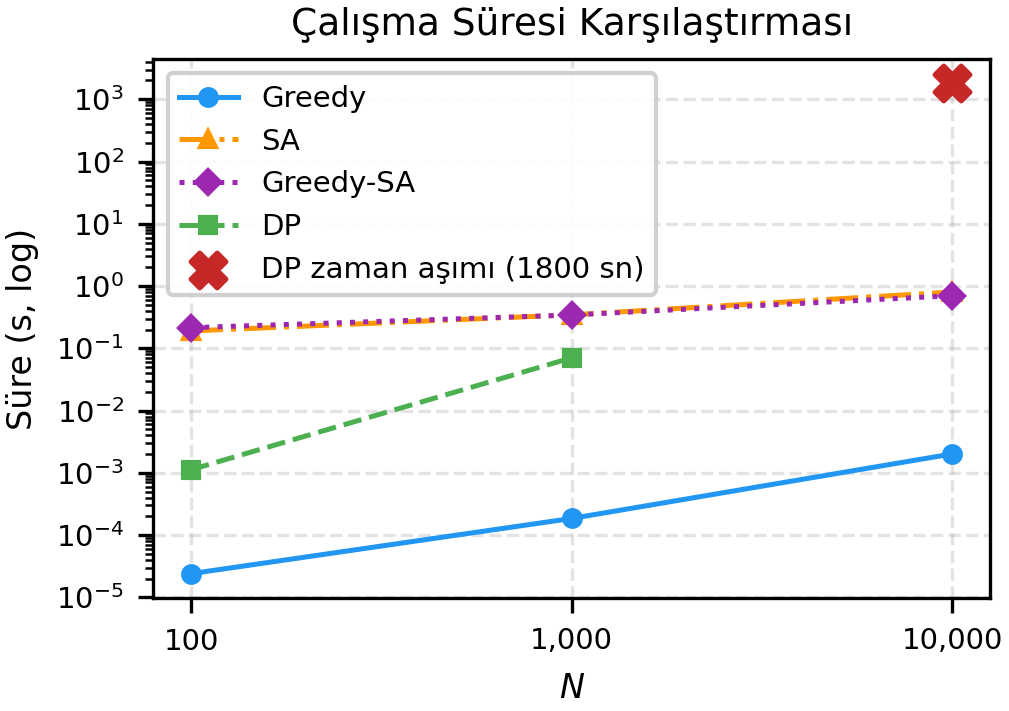
\includegraphics[width=0.95\columnwidth]{figures/runtime_comparison.png}
\caption{Algoritmaların çalışma süresi karşılaştırması.}
\label{fig:runtime}
\end{figure}

\subsection{Doğruluk Açığı}
Şekil~\ref{fig:accgap}, yalnızca $N{=}100$ ve $N{=}1000$ içindir; DP optimum referans iken SA, Greedy ve Greedy-SA için yüzde açık gösterilir. $N{=}10\,000$ grafikte yoktur (\texttt{timeout}; SA gap tanımsız).

\begin{figure}[!t]
\centering
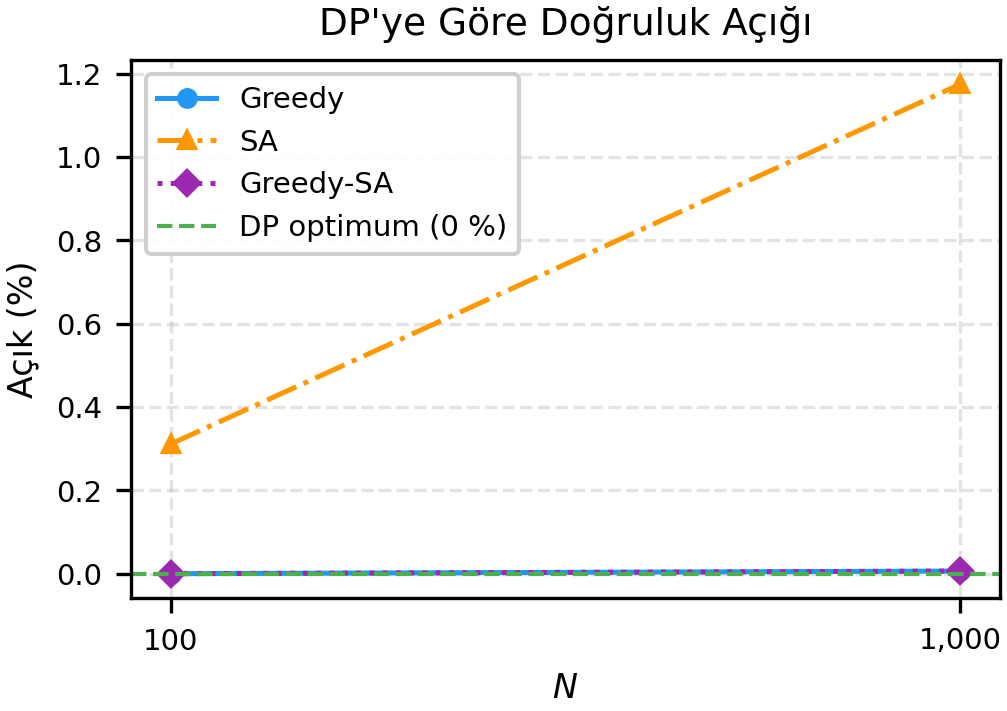
\includegraphics[width=0.95\columnwidth]{figures/accuracy_gap.png}
\caption{DP referansına göre doğruluk açığı.}
\label{fig:accgap}
\end{figure}

\subsection{DP Çalıştırma Durumu}
Şekil~\ref{fig:dpstatus}, her $N$ için DP'nin özet durumunu görselleştirir: $N{=}100$ ve $N{=}1000$ tamamlanma, $N{=}10\,000$ zaman aşımı.

\begin{figure}[!t]
\centering
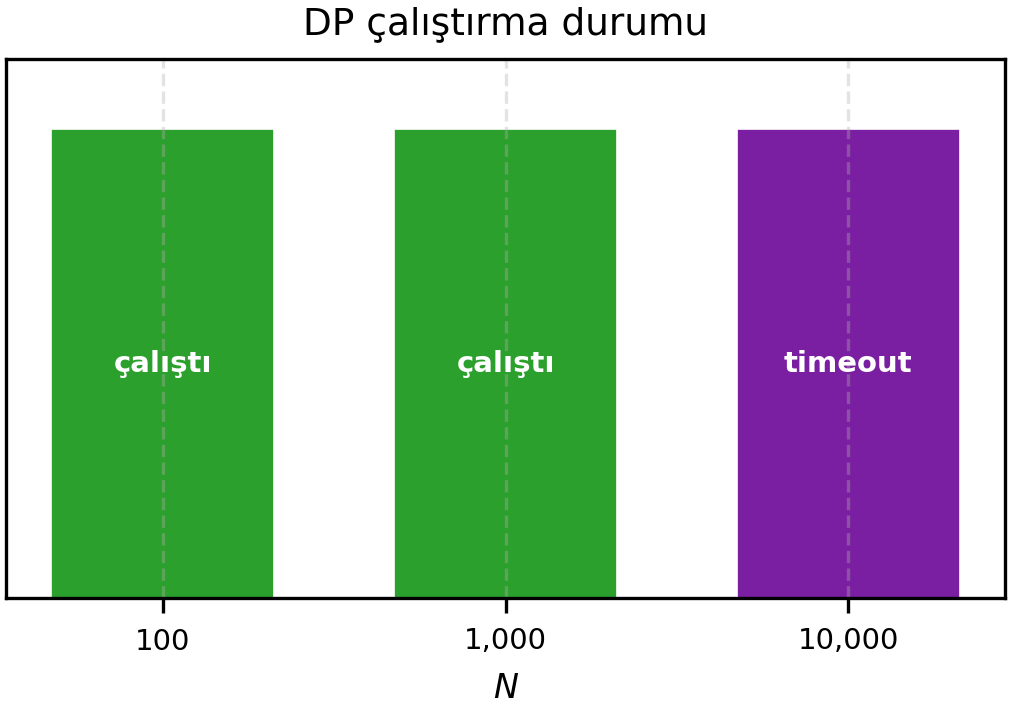
\includegraphics[width=0.95\columnwidth]{figures/dp_status_summary.png}
\caption{DP çalışma durumu.}
\label{fig:dpstatus}
\end{figure}

\FloatBarrier

\section{Sonuç}

Bu çalışma, proje isterindeki DP ve SA karşılaştırmasını sağlamaktadır. DP, $N{=}100$ ve $N{=}1000$ veri setlerinde optimum referans üretmiş; $N=10\,000$ veri setinde DP, yüksek hesaplama maliyeti ve CPU üzerinde uzun süren işlem yükü nedeniyle 1800 saniyelik süre sınırı içinde tamamlanamamıştır.

\vspace{-6pt}
\bibliographystyle{IEEEtran}
\bibliography{references}

\end{document}
